\documentclass[twoside]{book}

% Packages required by doxygen
\usepackage{fixltx2e}
\usepackage{calc}
\usepackage{doxygen}
\usepackage[export]{adjustbox} % also loads graphicx
\usepackage{graphicx}
\usepackage[utf8]{inputenc}
\usepackage{makeidx}
\usepackage{multicol}
\usepackage{multirow}
\PassOptionsToPackage{warn}{textcomp}
\usepackage{textcomp}
\usepackage[nointegrals]{wasysym}
\usepackage[table]{xcolor}

% Font selection
\usepackage[T1]{fontenc}
\usepackage[scaled=.90]{helvet}
\usepackage{courier}
\usepackage{amssymb}
\usepackage{sectsty}
\renewcommand{\familydefault}{\sfdefault}
\allsectionsfont{%
  \fontseries{bc}\selectfont%
  \color{darkgray}%
}
\renewcommand{\DoxyLabelFont}{%
  \fontseries{bc}\selectfont%
  \color{darkgray}%
}
\newcommand{\+}{\discretionary{\mbox{\scriptsize$\hookleftarrow$}}{}{}}

% Page & text layout
\usepackage{geometry}
\geometry{%
  a4paper,%
  top=2.5cm,%
  bottom=2.5cm,%
  left=2.5cm,%
  right=2.5cm%
}
\tolerance=750
\hfuzz=15pt
\hbadness=750
\setlength{\emergencystretch}{15pt}
\setlength{\parindent}{0cm}
\setlength{\parskip}{3ex plus 2ex minus 2ex}
\makeatletter
\renewcommand{\paragraph}{%
  \@startsection{paragraph}{4}{0ex}{-1.0ex}{1.0ex}{%
    \normalfont\normalsize\bfseries\SS@parafont%
  }%
}
\renewcommand{\subparagraph}{%
  \@startsection{subparagraph}{5}{0ex}{-1.0ex}{1.0ex}{%
    \normalfont\normalsize\bfseries\SS@subparafont%
  }%
}
\makeatother

% Headers & footers
\usepackage{fancyhdr}
\pagestyle{fancyplain}
\fancyhead[LE]{\fancyplain{}{\bfseries\thepage}}
\fancyhead[CE]{\fancyplain{}{}}
\fancyhead[RE]{\fancyplain{}{\bfseries\leftmark}}
\fancyhead[LO]{\fancyplain{}{\bfseries\rightmark}}
\fancyhead[CO]{\fancyplain{}{}}
\fancyhead[RO]{\fancyplain{}{\bfseries\thepage}}
\fancyfoot[LE]{\fancyplain{}{}}
\fancyfoot[CE]{\fancyplain{}{}}
\fancyfoot[RE]{\fancyplain{}{\bfseries\scriptsize Generated by Doxygen }}
\fancyfoot[LO]{\fancyplain{}{\bfseries\scriptsize Generated by Doxygen }}
\fancyfoot[CO]{\fancyplain{}{}}
\fancyfoot[RO]{\fancyplain{}{}}
\renewcommand{\footrulewidth}{0.4pt}
\renewcommand{\chaptermark}[1]{%
  \markboth{#1}{}%
}
\renewcommand{\sectionmark}[1]{%
  \markright{\thesection\ #1}%
}

% Indices & bibliography
\usepackage{natbib}
\usepackage[titles]{tocloft}
\setcounter{tocdepth}{3}
\setcounter{secnumdepth}{5}
\makeindex

% Hyperlinks (required, but should be loaded last)
\usepackage{ifpdf}
\ifpdf
  \usepackage[pdftex,pagebackref=true]{hyperref}
\else
  \usepackage[ps2pdf,pagebackref=true]{hyperref}
\fi
\hypersetup{%
  colorlinks=true,%
  linkcolor=blue,%
  citecolor=blue,%
  unicode%
}

% Custom commands
\newcommand{\clearemptydoublepage}{%
  \newpage{\pagestyle{empty}\cleardoublepage}%
}

\usepackage{caption}
\captionsetup{labelsep=space,justification=centering,font={bf},singlelinecheck=off,skip=4pt,position=top}

%===== C O N T E N T S =====

\begin{document}

% Titlepage & ToC
\hypersetup{pageanchor=false,
             bookmarksnumbered=true,
             pdfencoding=unicode
            }
\pagenumbering{roman}
\begin{titlepage}
\vspace*{7cm}
\begin{center}%
{\Large Application Document }\\
\vspace*{1cm}
{\large Generated by Doxygen 1.8.11}\\
\end{center}
\end{titlepage}
\clearemptydoublepage
\tableofcontents
\clearemptydoublepage
\pagenumbering{arabic}
\hypersetup{pageanchor=true}

%--- Begin generated contents ---
\chapter{The 2019-\/n\+CoV Prediction Application}
\label{index}\hypertarget{index}{}the 2019\+\_\+n\+CoV prediction application main node \begin{DoxyAuthor}{Author}
Peripatetic\+Wind (\href{mailto:zhangzhihong@stu.xjtu.edu.cn}{\tt zhangzhihong@stu.\+xjtu.\+edu.\+cn}) 
\end{DoxyAuthor}
\begin{DoxyVersion}{Version}
1.\+0.\+0 
\end{DoxyVersion}
\begin{DoxyDate}{Date}
2020-\/02-\/10 22\+:42\+:35 
\end{DoxyDate}
\begin{DoxyParagraph}{Last\+Editor}
Peripatetic\+Wind 
\end{DoxyParagraph}
\begin{DoxyParagraph}{Last\+Edit\+Time}
2020-\/02-\/10 22\+:42\+:35 
\end{DoxyParagraph}
\begin{DoxyParagraph}{Email}
\href{mailto:zhangzhihong@stu.xjtu.edu.cn}{\tt zhangzhihong@stu.\+xjtu.\+edu.\+cn} 
\end{DoxyParagraph}
\begin{DoxyParagraph}{Company}
Xi\textquotesingle{}an Jiaotong University 
\end{DoxyParagraph}
\begin{DoxyRefDesc}{Todo}
\item[\hyperlink{todo__todo000001}{Todo}]
\begin{DoxyEnumerate}
\item to add the details of the change log 
\end{DoxyEnumerate}\end{DoxyRefDesc}
\begin{DoxyRefDesc}{Bug}
\item[\hyperlink{bug__bug000001}{Bug}]
\begin{DoxyEnumerate}
\item the date will be wrong if no data of current day 
\end{DoxyEnumerate}\end{DoxyRefDesc}
\hypertarget{index_introduction_ection}{}\section{Introduction}\label{index_introduction_ection}
2019\+\_\+n\+CoV 每日感染人数预测程序 \hypertarget{index_dependencies_section}{}\section{Dependencies}\label{index_dependencies_section}

\begin{DoxyEnumerate}
\item 用到的\+C++相关库\+: G2O G\+L\+OG(含youibot log system) G\+F\+L\+A\+GS
\item 用到的python功能包\+: math matplotlib 
\end{DoxyEnumerate}\hypertarget{index_note_section}{}\section{Note Items}\label{index_note_section}

\begin{DoxyEnumerate}
\item 计算机上需要预先安装\+G2\+O。
\item 日志系统使用的是公司的日志系统,暂不开源,请谅解。如果要在自己的计算机上运行,可将代码中的日志替换为\+C++标准输出{\ttfamily std\+::cout$<$$<$},并取消main中\+Glogger对象的定义即可。 
\end{DoxyEnumerate}\hypertarget{index_install_section}{}\section{Installation}\label{index_install_section}
Just as the follows \hypertarget{index_step1}{}\subsection{Step 1\+: install g2o and youibot log system from github}\label{index_step1}
\hypertarget{index_step2}{}\subsection{Step 2\+: install math and matplotlib packages for python}\label{index_step2}
\hypertarget{index_step3}{}\subsection{Step 3\+: install the application}\label{index_step3}

\begin{DoxyCode}
$ cd 2019\_nCoV\_prediction
$ mkdir build
$ cd build
$ cmake ..
$ make
\end{DoxyCode}
 \begin{DoxyCopyright}{Copyright}
Copyright (c) 2020 Peripatetic\+Wind. All rights reserved. 
\end{DoxyCopyright}
\begin{DoxyParagraph}{License}
Licensed under the M\+IT License. 
\end{DoxyParagraph}
\begin{DoxyParagraph}{Changelog}

\tabulinesep=1mm
\begin{longtabu} spread 0pt [c]{*4{|X[-1]}|}
\caption{Change Log}\label{_}\\
\hline
\rowcolor{\tableheadbgcolor}{\bf Date }&{\bf Version }&{\bf Author }&{\bf Description }\\\cline{1-4}
\endfirsthead
\hline
\endfoot
\hline
\rowcolor{\tableheadbgcolor}{\bf Date }&{\bf Version }&{\bf Author }&{\bf Description }\\\cline{1-4}
\endhead
2020-\/02-\/10 22\+:42\+:35 &1.\+0.\+0 &Peripatetic\+Wind &change log \\\cline{1-4}
\end{longtabu}

\end{DoxyParagraph}

\chapter{Todo List}
\label{todo}
\hypertarget{todo}{}

\begin{DoxyRefList}
\item[\label{todo__todo000001}%
\hypertarget{todo__todo000001}{}%
page \hyperlink{index}{The 2019-\/n\+CoV Prediction Application} ]
\begin{DoxyEnumerate}
\item to add the details of the change log 
\end{DoxyEnumerate}
\end{DoxyRefList}
\chapter{Bug List}
\label{bug}
\hypertarget{bug}{}

\begin{DoxyRefList}
\item[\label{bug__bug000001}%
\hypertarget{bug__bug000001}{}%
page \hyperlink{index}{The 2019-\/n\+CoV Prediction Application} ]
\begin{DoxyEnumerate}
\item the date will be wrong if no data of current day 
\end{DoxyEnumerate}
\end{DoxyRefList}
\chapter{Hierarchical Index}
\section{Class Hierarchy}
This inheritance list is sorted roughly, but not completely, alphabetically\+:\begin{DoxyCompactList}
\item Base\+Unary\+Edge\begin{DoxyCompactList}
\item \contentsline{section}{Curve\+Fitting\+Edge}{\pageref{classCurveFittingEdge}}{}
\end{DoxyCompactList}
\item Base\+Vertex\begin{DoxyCompactList}
\item \contentsline{section}{Curve\+Fitting\+Vertex}{\pageref{classCurveFittingVertex}}{}
\end{DoxyCompactList}
\item \contentsline{section}{n\+CoV}{\pageref{classnCoV}}{}
\end{DoxyCompactList}

\chapter{Class Index}
\section{Class List}
Here are the classes, structs, unions and interfaces with brief descriptions\+:\begin{DoxyCompactList}
\item\contentsline{section}{\hyperlink{classCurveFittingEdge}{Curve\+Fitting\+Edge} }{\pageref{classCurveFittingEdge}}{}
\item\contentsline{section}{\hyperlink{classCurveFittingVertex}{Curve\+Fitting\+Vertex} }{\pageref{classCurveFittingVertex}}{}
\item\contentsline{section}{\hyperlink{classnCoV}{n\+CoV} }{\pageref{classnCoV}}{}
\end{DoxyCompactList}

\chapter{File Index}
\section{File List}
Here is a list of all files with brief descriptions\+:\begin{DoxyCompactList}
\item\contentsline{section}{include/\hyperlink{curve__fitting__edge_8h}{curve\+\_\+fitting\+\_\+edge.\+h} \\*The G2O model\textquotesingle{}s edge implementation file }{\pageref{curve__fitting__edge_8h}}{}
\item\contentsline{section}{include/\hyperlink{curve__fitting__vertex_8h}{curve\+\_\+fitting\+\_\+vertex.\+h} \\*The G2O model\textquotesingle{}s vertex implementation file }{\pageref{curve__fitting__vertex_8h}}{}
\item\contentsline{section}{include/\hyperlink{nCoV_8h}{n\+Co\+V.\+h} \\*N\+CoV class declaration file }{\pageref{nCoV_8h}}{}
\item\contentsline{section}{src/\hyperlink{main_8cpp}{main.\+cpp} \\*2019\+\_\+n\+CoV prediction program main node }{\pageref{main_8cpp}}{}
\item\contentsline{section}{src/\hyperlink{nCoV_8cpp}{n\+Co\+V.\+cpp} \\*N\+CoV class implementation file }{\pageref{nCoV_8cpp}}{}
\end{DoxyCompactList}

\chapter{Class Documentation}
\hypertarget{classCurveFittingEdge}{}\section{Curve\+Fitting\+Edge Class Reference}
\label{classCurveFittingEdge}\index{Curve\+Fitting\+Edge@{Curve\+Fitting\+Edge}}


\hyperlink{classCurveFittingEdge}{Curve\+Fitting\+Edge} g2o图优化模型的边类  




{\ttfamily \#include $<$curve\+\_\+fitting\+\_\+edge.\+h$>$}



Inheritance diagram for Curve\+Fitting\+Edge\+:\nopagebreak
\begin{figure}[H]
\begin{center}
\leavevmode
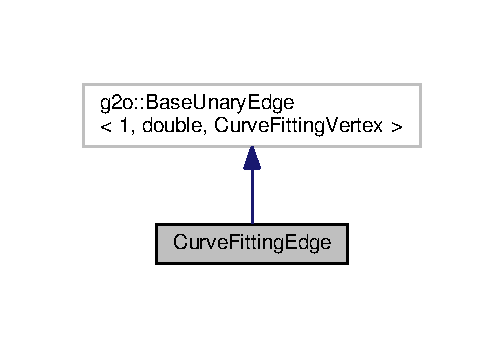
\includegraphics[width=242pt]{classCurveFittingEdge__inherit__graph}
\end{center}
\end{figure}


Collaboration diagram for Curve\+Fitting\+Edge\+:\nopagebreak
\begin{figure}[H]
\begin{center}
\leavevmode
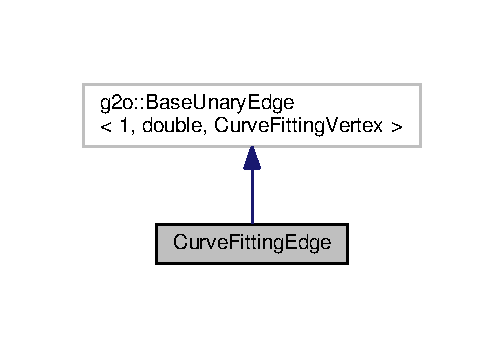
\includegraphics[width=242pt]{classCurveFittingEdge__coll__graph}
\end{center}
\end{figure}
\subsection*{Public Member Functions}
\begin{DoxyCompactItemize}
\item 
E\+I\+G\+E\+N\+\_\+\+M\+A\+K\+E\+\_\+\+A\+L\+I\+G\+N\+E\+D\+\_\+\+O\+P\+E\+R\+A\+T\+O\+R\+\_\+\+N\+EW \hyperlink{classCurveFittingEdge_a3a7ee01bc38a44a179faa78d78bcdc0b}{Curve\+Fitting\+Edge} (double x)
\begin{DoxyCompactList}\small\item\em G2\+O边模型构造函数 \end{DoxyCompactList}\item 
virtual void \hyperlink{classCurveFittingEdge_a4497b29e2f168d877d7a858457b69fd1}{compute\+Error} () override
\begin{DoxyCompactList}\small\item\em 计算曲线模型误差 \end{DoxyCompactList}\item 
virtual bool \hyperlink{classCurveFittingEdge_a517490d29ac656c6a0fc100b1af7cd9f}{read} (std\+::istream \&in) override
\begin{DoxyCompactList}\small\item\em 读盘,留空 \end{DoxyCompactList}\item 
virtual bool \hyperlink{classCurveFittingEdge_a70bde4a6cbed5fc825a069c6f1f45caa}{write} (std\+::ostream \&out) const override
\begin{DoxyCompactList}\small\item\em 存盘,留空 \end{DoxyCompactList}\end{DoxyCompactItemize}
\subsection*{Private Attributes}
\begin{DoxyCompactItemize}
\item 
double \hyperlink{classCurveFittingEdge_ad0cf7b012c9e4585a6919b982f148449}{\+\_\+x}
\begin{DoxyCompactList}\small\item\em x的值 y的值为\+\_\+measurement \end{DoxyCompactList}\end{DoxyCompactItemize}


\subsection{Detailed Description}
\hyperlink{classCurveFittingEdge}{Curve\+Fitting\+Edge} g2o图优化模型的边类 

g2o图优化模型的边类,定义残差计算规则和模型的自变量 

\subsection{Constructor \& Destructor Documentation}
\index{Curve\+Fitting\+Edge@{Curve\+Fitting\+Edge}!Curve\+Fitting\+Edge@{Curve\+Fitting\+Edge}}
\index{Curve\+Fitting\+Edge@{Curve\+Fitting\+Edge}!Curve\+Fitting\+Edge@{Curve\+Fitting\+Edge}}
\subsubsection[{\texorpdfstring{Curve\+Fitting\+Edge(double x)}{CurveFittingEdge(double x)}}]{\setlength{\rightskip}{0pt plus 5cm}E\+I\+G\+E\+N\+\_\+\+M\+A\+K\+E\+\_\+\+A\+L\+I\+G\+N\+E\+D\+\_\+\+O\+P\+E\+R\+A\+T\+O\+R\+\_\+\+N\+EW Curve\+Fitting\+Edge\+::\+Curve\+Fitting\+Edge (
\begin{DoxyParamCaption}
\item[{double}]{x}
\end{DoxyParamCaption}
)\hspace{0.3cm}{\ttfamily [inline]}}\hypertarget{classCurveFittingEdge_a3a7ee01bc38a44a179faa78d78bcdc0b}{}\label{classCurveFittingEdge_a3a7ee01bc38a44a179faa78d78bcdc0b}


G2\+O边模型构造函数 

Construct a new Curve Fitting Edge object


\begin{DoxyParams}[1]{Parameters}
\mbox{\tt in}  & {\em x} & 模型自变量x \\
\hline
\end{DoxyParams}


\subsection{Member Function Documentation}
\index{Curve\+Fitting\+Edge@{Curve\+Fitting\+Edge}!compute\+Error@{compute\+Error}}
\index{compute\+Error@{compute\+Error}!Curve\+Fitting\+Edge@{Curve\+Fitting\+Edge}}
\subsubsection[{\texorpdfstring{compute\+Error() override}{computeError() override}}]{\setlength{\rightskip}{0pt plus 5cm}virtual void Curve\+Fitting\+Edge\+::compute\+Error (
\begin{DoxyParamCaption}
{}
\end{DoxyParamCaption}
)\hspace{0.3cm}{\ttfamily [inline]}, {\ttfamily [override]}, {\ttfamily [virtual]}}\hypertarget{classCurveFittingEdge_a4497b29e2f168d877d7a858457b69fd1}{}\label{classCurveFittingEdge_a4497b29e2f168d877d7a858457b69fd1}


计算曲线模型误差 

\index{Curve\+Fitting\+Edge@{Curve\+Fitting\+Edge}!read@{read}}
\index{read@{read}!Curve\+Fitting\+Edge@{Curve\+Fitting\+Edge}}
\subsubsection[{\texorpdfstring{read(std\+::istream \&in) override}{read(std::istream &in) override}}]{\setlength{\rightskip}{0pt plus 5cm}virtual bool Curve\+Fitting\+Edge\+::read (
\begin{DoxyParamCaption}
\item[{std\+::istream \&}]{in}
\end{DoxyParamCaption}
)\hspace{0.3cm}{\ttfamily [inline]}, {\ttfamily [override]}, {\ttfamily [virtual]}}\hypertarget{classCurveFittingEdge_a517490d29ac656c6a0fc100b1af7cd9f}{}\label{classCurveFittingEdge_a517490d29ac656c6a0fc100b1af7cd9f}


读盘,留空 

\index{Curve\+Fitting\+Edge@{Curve\+Fitting\+Edge}!write@{write}}
\index{write@{write}!Curve\+Fitting\+Edge@{Curve\+Fitting\+Edge}}
\subsubsection[{\texorpdfstring{write(std\+::ostream \&out) const override}{write(std::ostream &out) const override}}]{\setlength{\rightskip}{0pt plus 5cm}virtual bool Curve\+Fitting\+Edge\+::write (
\begin{DoxyParamCaption}
\item[{std\+::ostream \&}]{out}
\end{DoxyParamCaption}
) const\hspace{0.3cm}{\ttfamily [inline]}, {\ttfamily [override]}, {\ttfamily [virtual]}}\hypertarget{classCurveFittingEdge_a70bde4a6cbed5fc825a069c6f1f45caa}{}\label{classCurveFittingEdge_a70bde4a6cbed5fc825a069c6f1f45caa}


存盘,留空 



\subsection{Member Data Documentation}
\index{Curve\+Fitting\+Edge@{Curve\+Fitting\+Edge}!\+\_\+x@{\+\_\+x}}
\index{\+\_\+x@{\+\_\+x}!Curve\+Fitting\+Edge@{Curve\+Fitting\+Edge}}
\subsubsection[{\texorpdfstring{\+\_\+x}{_x}}]{\setlength{\rightskip}{0pt plus 5cm}double Curve\+Fitting\+Edge\+::\+\_\+x\hspace{0.3cm}{\ttfamily [private]}}\hypertarget{classCurveFittingEdge_ad0cf7b012c9e4585a6919b982f148449}{}\label{classCurveFittingEdge_ad0cf7b012c9e4585a6919b982f148449}


x的值 y的值为\+\_\+measurement 



The documentation for this class was generated from the following file\+:\begin{DoxyCompactItemize}
\item 
include/\hyperlink{curve__fitting__edge_8h}{curve\+\_\+fitting\+\_\+edge.\+h}\end{DoxyCompactItemize}

\hypertarget{classCurveFittingVertex}{}\section{Curve\+Fitting\+Vertex Class Reference}
\label{classCurveFittingVertex}\index{Curve\+Fitting\+Vertex@{Curve\+Fitting\+Vertex}}


\hyperlink{classCurveFittingVertex}{Curve\+Fitting\+Vertex} g2o图优化模型的顶点类  




{\ttfamily \#include $<$curve\+\_\+fitting\+\_\+vertex.\+h$>$}



Inheritance diagram for Curve\+Fitting\+Vertex\+:\nopagebreak
\begin{figure}[H]
\begin{center}
\leavevmode
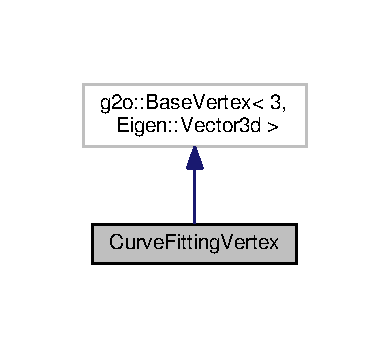
\includegraphics[width=187pt]{classCurveFittingVertex__inherit__graph}
\end{center}
\end{figure}


Collaboration diagram for Curve\+Fitting\+Vertex\+:\nopagebreak
\begin{figure}[H]
\begin{center}
\leavevmode
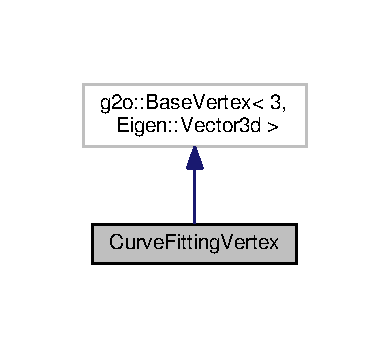
\includegraphics[width=187pt]{classCurveFittingVertex__coll__graph}
\end{center}
\end{figure}
\subsection*{Public Member Functions}
\begin{DoxyCompactItemize}
\item 
virtual E\+I\+G\+E\+N\+\_\+\+M\+A\+K\+E\+\_\+\+A\+L\+I\+G\+N\+E\+D\+\_\+\+O\+P\+E\+R\+A\+T\+O\+R\+\_\+\+N\+EW void \hyperlink{classCurveFittingVertex_a47ac379f177a871d1352c1c9dc64fa16}{set\+To\+Origin\+Impl} () override
\begin{DoxyCompactList}\small\item\em Set the To Origin Impl object. \end{DoxyCompactList}\item 
virtual void \hyperlink{classCurveFittingVertex_a4e384a35c5f108f2ca7fbcad204c4df3}{oplus\+Impl} (const double $\ast$update) override
\begin{DoxyCompactList}\small\item\em 设置顶点的更新规则 update为更新量 \end{DoxyCompactList}\item 
virtual bool \hyperlink{classCurveFittingVertex_aa96dd0a2d3d3bfe757484c912dd0f27b}{read} (std\+::istream \&in) override
\begin{DoxyCompactList}\small\item\em 读盘,留空 \end{DoxyCompactList}\item 
virtual bool \hyperlink{classCurveFittingVertex_aa1443355babb211e227422ea0675dc32}{write} (std\+::ostream \&out) const override
\begin{DoxyCompactList}\small\item\em 存盘,留空 \end{DoxyCompactList}\end{DoxyCompactItemize}


\subsection{Detailed Description}
\hyperlink{classCurveFittingVertex}{Curve\+Fitting\+Vertex} g2o图优化模型的顶点类 

g2o图优化模型的顶点类,设置初值,以及顶点更新规则 

\subsection{Member Function Documentation}
\index{Curve\+Fitting\+Vertex@{Curve\+Fitting\+Vertex}!oplus\+Impl@{oplus\+Impl}}
\index{oplus\+Impl@{oplus\+Impl}!Curve\+Fitting\+Vertex@{Curve\+Fitting\+Vertex}}
\subsubsection[{\texorpdfstring{oplus\+Impl(const double $\ast$update) override}{oplusImpl(const double *update) override}}]{\setlength{\rightskip}{0pt plus 5cm}virtual void Curve\+Fitting\+Vertex\+::oplus\+Impl (
\begin{DoxyParamCaption}
\item[{const double $\ast$}]{update}
\end{DoxyParamCaption}
)\hspace{0.3cm}{\ttfamily [inline]}, {\ttfamily [override]}, {\ttfamily [virtual]}}\hypertarget{classCurveFittingVertex_a4e384a35c5f108f2ca7fbcad204c4df3}{}\label{classCurveFittingVertex_a4e384a35c5f108f2ca7fbcad204c4df3}


设置顶点的更新规则 update为更新量 


\begin{DoxyParams}[1]{Parameters}
\mbox{\tt in}  & {\em update} & 更新变量 \\
\hline
\end{DoxyParams}
\index{Curve\+Fitting\+Vertex@{Curve\+Fitting\+Vertex}!read@{read}}
\index{read@{read}!Curve\+Fitting\+Vertex@{Curve\+Fitting\+Vertex}}
\subsubsection[{\texorpdfstring{read(std\+::istream \&in) override}{read(std::istream &in) override}}]{\setlength{\rightskip}{0pt plus 5cm}virtual bool Curve\+Fitting\+Vertex\+::read (
\begin{DoxyParamCaption}
\item[{std\+::istream \&}]{in}
\end{DoxyParamCaption}
)\hspace{0.3cm}{\ttfamily [inline]}, {\ttfamily [override]}, {\ttfamily [virtual]}}\hypertarget{classCurveFittingVertex_aa96dd0a2d3d3bfe757484c912dd0f27b}{}\label{classCurveFittingVertex_aa96dd0a2d3d3bfe757484c912dd0f27b}


读盘,留空 

\index{Curve\+Fitting\+Vertex@{Curve\+Fitting\+Vertex}!set\+To\+Origin\+Impl@{set\+To\+Origin\+Impl}}
\index{set\+To\+Origin\+Impl@{set\+To\+Origin\+Impl}!Curve\+Fitting\+Vertex@{Curve\+Fitting\+Vertex}}
\subsubsection[{\texorpdfstring{set\+To\+Origin\+Impl() override}{setToOriginImpl() override}}]{\setlength{\rightskip}{0pt plus 5cm}virtual E\+I\+G\+E\+N\+\_\+\+M\+A\+K\+E\+\_\+\+A\+L\+I\+G\+N\+E\+D\+\_\+\+O\+P\+E\+R\+A\+T\+O\+R\+\_\+\+N\+EW void Curve\+Fitting\+Vertex\+::set\+To\+Origin\+Impl (
\begin{DoxyParamCaption}
{}
\end{DoxyParamCaption}
)\hspace{0.3cm}{\ttfamily [inline]}, {\ttfamily [override]}, {\ttfamily [virtual]}}\hypertarget{classCurveFittingVertex_a47ac379f177a871d1352c1c9dc64fa16}{}\label{classCurveFittingVertex_a47ac379f177a871d1352c1c9dc64fa16}


Set the To Origin Impl object. 

\index{Curve\+Fitting\+Vertex@{Curve\+Fitting\+Vertex}!write@{write}}
\index{write@{write}!Curve\+Fitting\+Vertex@{Curve\+Fitting\+Vertex}}
\subsubsection[{\texorpdfstring{write(std\+::ostream \&out) const override}{write(std::ostream &out) const override}}]{\setlength{\rightskip}{0pt plus 5cm}virtual bool Curve\+Fitting\+Vertex\+::write (
\begin{DoxyParamCaption}
\item[{std\+::ostream \&}]{out}
\end{DoxyParamCaption}
) const\hspace{0.3cm}{\ttfamily [inline]}, {\ttfamily [override]}, {\ttfamily [virtual]}}\hypertarget{classCurveFittingVertex_aa1443355babb211e227422ea0675dc32}{}\label{classCurveFittingVertex_aa1443355babb211e227422ea0675dc32}


存盘,留空 



The documentation for this class was generated from the following file\+:\begin{DoxyCompactItemize}
\item 
include/\hyperlink{curve__fitting__vertex_8h}{curve\+\_\+fitting\+\_\+vertex.\+h}\end{DoxyCompactItemize}

\hypertarget{classnCoV}{}\section{n\+CoV Class Reference}
\label{classnCoV}\index{n\+CoV@{n\+CoV}}


\hyperlink{classnCoV}{n\+CoV} class  




{\ttfamily \#include $<$n\+Co\+V.\+h$>$}

\subsection*{Public Member Functions}
\begin{DoxyCompactItemize}
\item 
\hyperlink{classnCoV_a30d4a90c5f401cf6943e104ec737dc48}{n\+CoV} (int predict\+Days)
\begin{DoxyCompactList}\small\item\em \hyperlink{classnCoV}{n\+CoV} class,用以建立图模型并优化,最后预测 \end{DoxyCompactList}\end{DoxyCompactItemize}
\subsection*{Private Member Functions}
\begin{DoxyCompactItemize}
\item 
void \hyperlink{classnCoV_acf5ddd73cab8522622b2602258507c08}{optimize} ()
\begin{DoxyCompactList}\small\item\em 模型优化函数 \end{DoxyCompactList}\item 
void \hyperlink{classnCoV_a5a0b30d27da271601d45c144c6a3da2d}{predict} ()
\begin{DoxyCompactList}\small\item\em 模型预测函数 \end{DoxyCompactList}\end{DoxyCompactItemize}
\subsection*{Private Attributes}
\begin{DoxyCompactItemize}
\item 
int \hyperlink{classnCoV_a7182f86ff0f0f607cd461ebe738fb9da}{\+\_\+data\+Size}
\begin{DoxyCompactList}\small\item\em 数据量,每天1条数据,即为天数 \end{DoxyCompactList}\item 
int \hyperlink{classnCoV_a71d73f9132ff05684bb8f830bd1f4232}{\+\_\+predict\+Days}
\begin{DoxyCompactList}\small\item\em 要预测的天数 \end{DoxyCompactList}\item 
std\+::ifstream \hyperlink{classnCoV_a9585e58cac7c3c4cf26fe0291b809f06}{\+\_\+data\+File}
\begin{DoxyCompactList}\small\item\em 数据文件 \end{DoxyCompactList}\item 
std\+::vector$<$ double $>$ \hyperlink{classnCoV_a11802f3972f62a07b77b1847f1d010a8}{\+\_\+x\+Data}
\begin{DoxyCompactList}\small\item\em 优化模型的自变量,为每日日期 \end{DoxyCompactList}\item 
std\+::vector$<$ double $>$ \hyperlink{classnCoV_a8e122688ffc8ee32df05f0cb6ef25920}{\+\_\+y\+Data}
\begin{DoxyCompactList}\small\item\em 优化模型的因变量,为每日累计感染人数 \end{DoxyCompactList}\item 
double \hyperlink{classnCoV_ae34cb58fd08703599158b69853b659a2}{\+\_\+parameter} \mbox{[}3\mbox{]}
\begin{DoxyCompactList}\small\item\em 待优化的\+S\+I\+R模型参数的初值 \end{DoxyCompactList}\item 
Eigen\+::\+Vector3d \hyperlink{classnCoV_a6980bf4492a8ce437b15ac9625eacfce}{\+\_\+parameter\+Estimated}
\begin{DoxyCompactList}\small\item\em 优化后的\+S\+I\+R模型参数值 \end{DoxyCompactList}\end{DoxyCompactItemize}


\subsection{Detailed Description}
\hyperlink{classnCoV}{n\+CoV} class 

\hyperlink{classnCoV}{n\+CoV} class to optimaize the graph model and predict infected numbers 

\subsection{Constructor \& Destructor Documentation}
\index{n\+CoV@{n\+CoV}!n\+CoV@{n\+CoV}}
\index{n\+CoV@{n\+CoV}!n\+CoV@{n\+CoV}}
\subsubsection[{\texorpdfstring{n\+Co\+V(int predict\+Days)}{nCoV(int predictDays)}}]{\setlength{\rightskip}{0pt plus 5cm}n\+Co\+V\+::n\+CoV (
\begin{DoxyParamCaption}
\item[{int}]{predict\+Days}
\end{DoxyParamCaption}
)}\hypertarget{classnCoV_a30d4a90c5f401cf6943e104ec737dc48}{}\label{classnCoV_a30d4a90c5f401cf6943e104ec737dc48}


\hyperlink{classnCoV}{n\+CoV} class,用以建立图模型并优化,最后预测 

Construct a new \hyperlink{classnCoV_a30d4a90c5f401cf6943e104ec737dc48}{n\+Co\+V\+::n\+CoV} object


\begin{DoxyParams}[1]{Parameters}
\mbox{\tt in}  & {\em predict\+Days} & the days you want to predict \\
\hline
\end{DoxyParams}


\subsection{Member Function Documentation}
\index{n\+CoV@{n\+CoV}!optimize@{optimize}}
\index{optimize@{optimize}!n\+CoV@{n\+CoV}}
\subsubsection[{\texorpdfstring{optimize()}{optimize()}}]{\setlength{\rightskip}{0pt plus 5cm}void n\+Co\+V\+::optimize (
\begin{DoxyParamCaption}
{}
\end{DoxyParamCaption}
)\hspace{0.3cm}{\ttfamily [private]}}\hypertarget{classnCoV_acf5ddd73cab8522622b2602258507c08}{}\label{classnCoV_acf5ddd73cab8522622b2602258507c08}


模型优化函数 

G2\+O图模型优化

G2\+O图模型优化,用来建立\+S\+I\+R模型,优化该模型的参数值 \begin{DoxyPostcond}{Postcondition}
之后需要调用prediction函数进行预测 
\end{DoxyPostcond}
\index{n\+CoV@{n\+CoV}!predict@{predict}}
\index{predict@{predict}!n\+CoV@{n\+CoV}}
\subsubsection[{\texorpdfstring{predict()}{predict()}}]{\setlength{\rightskip}{0pt plus 5cm}void n\+Co\+V\+::predict (
\begin{DoxyParamCaption}
{}
\end{DoxyParamCaption}
)\hspace{0.3cm}{\ttfamily [private]}}\hypertarget{classnCoV_a5a0b30d27da271601d45c144c6a3da2d}{}\label{classnCoV_a5a0b30d27da271601d45c144c6a3da2d}


模型预测函数 

根据\+S\+I\+R模型,预测感染人数

根据图模型优化的参数,建立\+S\+I\+R模型,预测指定天数每天的感染人数 \begin{DoxyPrecond}{Precondition}
必须先调用optimize函数进行模型优化 
\end{DoxyPrecond}


\subsection{Member Data Documentation}
\index{n\+CoV@{n\+CoV}!\+\_\+data\+File@{\+\_\+data\+File}}
\index{\+\_\+data\+File@{\+\_\+data\+File}!n\+CoV@{n\+CoV}}
\subsubsection[{\texorpdfstring{\+\_\+data\+File}{_dataFile}}]{\setlength{\rightskip}{0pt plus 5cm}std\+::ifstream n\+Co\+V\+::\+\_\+data\+File\hspace{0.3cm}{\ttfamily [private]}}\hypertarget{classnCoV_a9585e58cac7c3c4cf26fe0291b809f06}{}\label{classnCoV_a9585e58cac7c3c4cf26fe0291b809f06}


数据文件 

\index{n\+CoV@{n\+CoV}!\+\_\+data\+Size@{\+\_\+data\+Size}}
\index{\+\_\+data\+Size@{\+\_\+data\+Size}!n\+CoV@{n\+CoV}}
\subsubsection[{\texorpdfstring{\+\_\+data\+Size}{_dataSize}}]{\setlength{\rightskip}{0pt plus 5cm}int n\+Co\+V\+::\+\_\+data\+Size\hspace{0.3cm}{\ttfamily [private]}}\hypertarget{classnCoV_a7182f86ff0f0f607cd461ebe738fb9da}{}\label{classnCoV_a7182f86ff0f0f607cd461ebe738fb9da}


数据量,每天1条数据,即为天数 

\index{n\+CoV@{n\+CoV}!\+\_\+parameter@{\+\_\+parameter}}
\index{\+\_\+parameter@{\+\_\+parameter}!n\+CoV@{n\+CoV}}
\subsubsection[{\texorpdfstring{\+\_\+parameter}{_parameter}}]{\setlength{\rightskip}{0pt plus 5cm}double n\+Co\+V\+::\+\_\+parameter\mbox{[}3\mbox{]}\hspace{0.3cm}{\ttfamily [private]}}\hypertarget{classnCoV_ae34cb58fd08703599158b69853b659a2}{}\label{classnCoV_ae34cb58fd08703599158b69853b659a2}


待优化的\+S\+I\+R模型参数的初值 

\index{n\+CoV@{n\+CoV}!\+\_\+parameter\+Estimated@{\+\_\+parameter\+Estimated}}
\index{\+\_\+parameter\+Estimated@{\+\_\+parameter\+Estimated}!n\+CoV@{n\+CoV}}
\subsubsection[{\texorpdfstring{\+\_\+parameter\+Estimated}{_parameterEstimated}}]{\setlength{\rightskip}{0pt plus 5cm}Eigen\+::\+Vector3d n\+Co\+V\+::\+\_\+parameter\+Estimated\hspace{0.3cm}{\ttfamily [private]}}\hypertarget{classnCoV_a6980bf4492a8ce437b15ac9625eacfce}{}\label{classnCoV_a6980bf4492a8ce437b15ac9625eacfce}


优化后的\+S\+I\+R模型参数值 

\index{n\+CoV@{n\+CoV}!\+\_\+predict\+Days@{\+\_\+predict\+Days}}
\index{\+\_\+predict\+Days@{\+\_\+predict\+Days}!n\+CoV@{n\+CoV}}
\subsubsection[{\texorpdfstring{\+\_\+predict\+Days}{_predictDays}}]{\setlength{\rightskip}{0pt plus 5cm}int n\+Co\+V\+::\+\_\+predict\+Days\hspace{0.3cm}{\ttfamily [private]}}\hypertarget{classnCoV_a71d73f9132ff05684bb8f830bd1f4232}{}\label{classnCoV_a71d73f9132ff05684bb8f830bd1f4232}


要预测的天数 

\index{n\+CoV@{n\+CoV}!\+\_\+x\+Data@{\+\_\+x\+Data}}
\index{\+\_\+x\+Data@{\+\_\+x\+Data}!n\+CoV@{n\+CoV}}
\subsubsection[{\texorpdfstring{\+\_\+x\+Data}{_xData}}]{\setlength{\rightskip}{0pt plus 5cm}std\+::vector$<$double$>$ n\+Co\+V\+::\+\_\+x\+Data\hspace{0.3cm}{\ttfamily [private]}}\hypertarget{classnCoV_a11802f3972f62a07b77b1847f1d010a8}{}\label{classnCoV_a11802f3972f62a07b77b1847f1d010a8}


优化模型的自变量,为每日日期 

\index{n\+CoV@{n\+CoV}!\+\_\+y\+Data@{\+\_\+y\+Data}}
\index{\+\_\+y\+Data@{\+\_\+y\+Data}!n\+CoV@{n\+CoV}}
\subsubsection[{\texorpdfstring{\+\_\+y\+Data}{_yData}}]{\setlength{\rightskip}{0pt plus 5cm}std\+::vector$<$double$>$ n\+Co\+V\+::\+\_\+y\+Data\hspace{0.3cm}{\ttfamily [private]}}\hypertarget{classnCoV_a8e122688ffc8ee32df05f0cb6ef25920}{}\label{classnCoV_a8e122688ffc8ee32df05f0cb6ef25920}


优化模型的因变量,为每日累计感染人数 



The documentation for this class was generated from the following files\+:\begin{DoxyCompactItemize}
\item 
include/\hyperlink{nCoV_8h}{n\+Co\+V.\+h}\item 
src/\hyperlink{nCoV_8cpp}{n\+Co\+V.\+cpp}\end{DoxyCompactItemize}

\chapter{File Documentation}
\hypertarget{curve__fitting__edge_8h}{}\section{include/curve\+\_\+fitting\+\_\+edge.h File Reference}
\label{curve__fitting__edge_8h}\index{include/curve\+\_\+fitting\+\_\+edge.\+h@{include/curve\+\_\+fitting\+\_\+edge.\+h}}


The G2O model\textquotesingle{}s edge implementation file.  


{\ttfamily \#include $<$iostream$>$}\\*
{\ttfamily \#include $<$Eigen/\+Core$>$}\\*
{\ttfamily \#include $<$g2o/core/base\+\_\+unary\+\_\+edge.\+h$>$}\\*
{\ttfamily \#include \char`\"{}curve\+\_\+fitting\+\_\+vertex.\+h\char`\"{}}\\*
Include dependency graph for curve\+\_\+fitting\+\_\+edge.\+h\+:\nopagebreak
\begin{figure}[H]
\begin{center}
\leavevmode
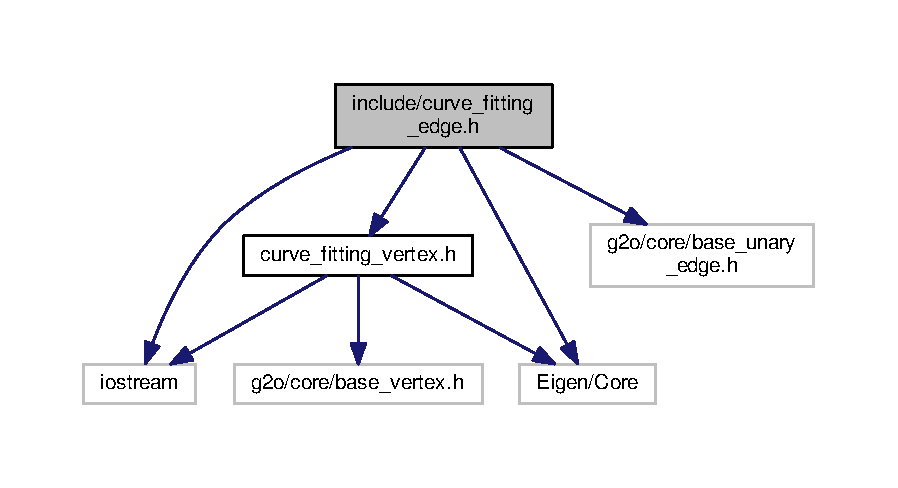
\includegraphics[width=350pt]{curve__fitting__edge_8h__incl}
\end{center}
\end{figure}
This graph shows which files directly or indirectly include this file\+:\nopagebreak
\begin{figure}[H]
\begin{center}
\leavevmode
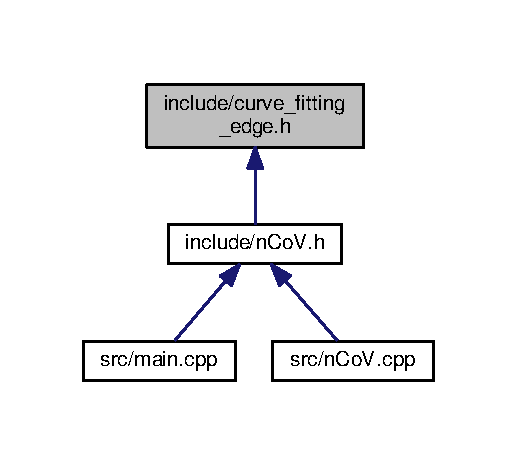
\includegraphics[width=248pt]{curve__fitting__edge_8h__dep__incl}
\end{center}
\end{figure}
\subsection*{Classes}
\begin{DoxyCompactItemize}
\item 
class \hyperlink{classCurveFittingEdge}{Curve\+Fitting\+Edge}
\end{DoxyCompactItemize}


\subsection{Detailed Description}
The G2O model\textquotesingle{}s edge implementation file. 

\begin{DoxyAuthor}{Author}
Peripatetic\+Wind (\href{mailto:zhangzhihong@stu.xjtu.edu.cn}{\tt zhangzhihong@stu.\+xjtu.\+edu.\+cn}) 
\end{DoxyAuthor}
\begin{DoxyVersion}{Version}
1.\+0.\+0 
\end{DoxyVersion}
\begin{DoxyDate}{Date}
2020-\/02-\/10 22\+:44\+:06 
\end{DoxyDate}
\begin{DoxyParagraph}{Last\+Editor}
Peripatetic\+Wind 
\end{DoxyParagraph}
\begin{DoxyParagraph}{Last\+Edit\+Time}
2020-\/02-\/10 22\+:44\+:06 
\end{DoxyParagraph}
\begin{DoxyParagraph}{Email}
\href{mailto:zhangzhihong@stu.xjtu.edu.cn}{\tt zhangzhihong@stu.\+xjtu.\+edu.\+cn} 
\end{DoxyParagraph}
\begin{DoxyParagraph}{Company}
Xi\textquotesingle{}an Jiaotong University 
\end{DoxyParagraph}
\begin{DoxyCopyright}{Copyright}
Copyright (c) 2020 Peripatetic\+Wind. All rights reserved. 
\end{DoxyCopyright}
\begin{DoxyParagraph}{License}
Licensed under the M\+IT License. 
\end{DoxyParagraph}
\begin{DoxyParagraph}{Changelog}

\tabulinesep=1mm
\begin{longtabu} spread 0pt [c]{*4{|X[-1]}|}
\caption{Change Log}\label{_}\\
\hline
\rowcolor{\tableheadbgcolor}{\bf Date }&{\bf Version }&{\bf Author }&{\bf Description }\\\cline{1-4}
\endfirsthead
\hline
\endfoot
\hline
\rowcolor{\tableheadbgcolor}{\bf Date }&{\bf Version }&{\bf Author }&{\bf Description }\\\cline{1-4}
\endhead
2020-\/02-\/10 22\+:44\+:06 &1.\+0.\+0 &Peripatetic\+Wind &change log \\\cline{1-4}
\end{longtabu}

\end{DoxyParagraph}

\hypertarget{curve__fitting__vertex_8h}{}\section{include/curve\+\_\+fitting\+\_\+vertex.h File Reference}
\label{curve__fitting__vertex_8h}\index{include/curve\+\_\+fitting\+\_\+vertex.\+h@{include/curve\+\_\+fitting\+\_\+vertex.\+h}}


The G2O model\textquotesingle{}s vertex implementation file.  


{\ttfamily \#include $<$iostream$>$}\\*
{\ttfamily \#include $<$Eigen/\+Core$>$}\\*
{\ttfamily \#include $<$g2o/core/base\+\_\+vertex.\+h$>$}\\*
Include dependency graph for curve\+\_\+fitting\+\_\+vertex.\+h\+:\nopagebreak
\begin{figure}[H]
\begin{center}
\leavevmode
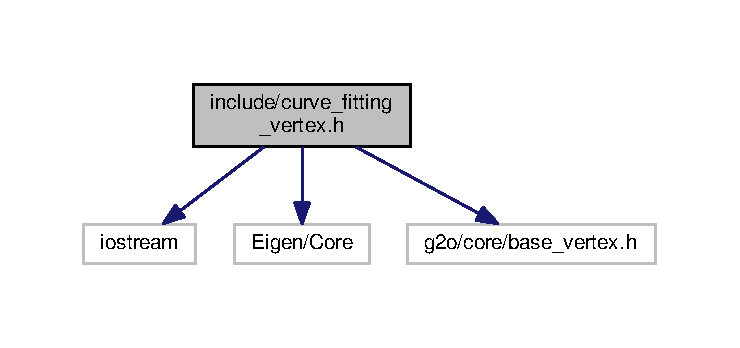
\includegraphics[width=350pt]{curve__fitting__vertex_8h__incl}
\end{center}
\end{figure}
This graph shows which files directly or indirectly include this file\+:\nopagebreak
\begin{figure}[H]
\begin{center}
\leavevmode
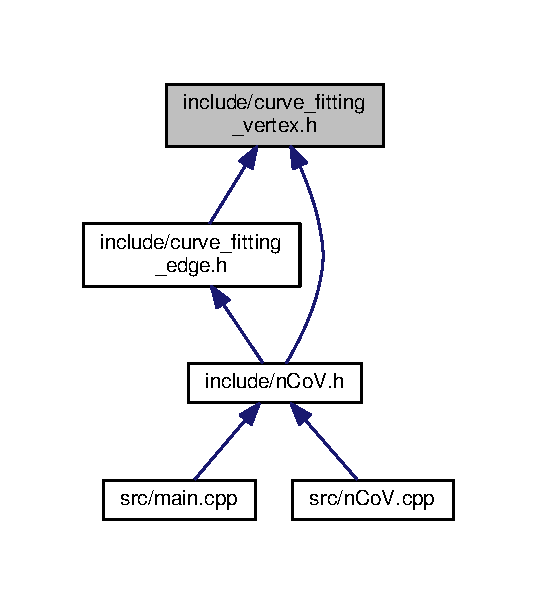
\includegraphics[width=258pt]{curve__fitting__vertex_8h__dep__incl}
\end{center}
\end{figure}
\subsection*{Classes}
\begin{DoxyCompactItemize}
\item 
class \hyperlink{classCurveFittingVertex}{Curve\+Fitting\+Vertex}
\begin{DoxyCompactList}\small\item\em \hyperlink{classCurveFittingVertex}{Curve\+Fitting\+Vertex} g2o图优化模型的顶点类 \end{DoxyCompactList}\end{DoxyCompactItemize}


\subsection{Detailed Description}
The G2O model\textquotesingle{}s vertex implementation file. 

\begin{DoxyAuthor}{Author}
Peripatetic\+Wind (\href{mailto:zhangzhihong@stu.xjtu.edu.cn}{\tt zhangzhihong@stu.\+xjtu.\+edu.\+cn}) 
\end{DoxyAuthor}
\begin{DoxyVersion}{Version}
1.\+0.\+0 
\end{DoxyVersion}
\begin{DoxyDate}{Date}
2020-\/02-\/10 22\+:43\+:51 
\end{DoxyDate}
\begin{DoxyParagraph}{Last\+Editor}
Peripatetic\+Wind 
\end{DoxyParagraph}
\begin{DoxyParagraph}{Last\+Edit\+Time}
2020-\/02-\/10 22\+:43\+:51 
\end{DoxyParagraph}
\begin{DoxyParagraph}{Email}
\href{mailto:zhangzhihong@stu.xjtu.edu.cn}{\tt zhangzhihong@stu.\+xjtu.\+edu.\+cn} 
\end{DoxyParagraph}
\begin{DoxyParagraph}{Company}
Xi\textquotesingle{}an Jiaotong University 
\end{DoxyParagraph}
\begin{DoxyCopyright}{Copyright}
Copyright (c) 2020 Peripatetic\+Wind. All rights reserved. 
\end{DoxyCopyright}
\begin{DoxyParagraph}{License}
Licensed under the M\+IT License. 
\end{DoxyParagraph}
\begin{DoxyParagraph}{Changelog}

\tabulinesep=1mm
\begin{longtabu} spread 0pt [c]{*4{|X[-1]}|}
\caption{Change Log}\label{_}\\
\hline
\rowcolor{\tableheadbgcolor}{\bf Date }&{\bf Version }&{\bf Author }&{\bf Description }\\\cline{1-4}
\endfirsthead
\hline
\endfoot
\hline
\rowcolor{\tableheadbgcolor}{\bf Date }&{\bf Version }&{\bf Author }&{\bf Description }\\\cline{1-4}
\endhead
2020-\/02-\/10 22\+:43\+:51 &1.\+0.\+0 &Peripatetic\+Wind &change log \\\cline{1-4}
\end{longtabu}

\end{DoxyParagraph}

\hypertarget{nCoV_8h}{}\section{include/n\+CoV.h File Reference}
\label{nCoV_8h}\index{include/n\+Co\+V.\+h@{include/n\+Co\+V.\+h}}


the \hyperlink{classnCoV}{n\+CoV} class declaration file  


{\ttfamily \#include $<$algorithm$>$}\\*
{\ttfamily \#include $<$chrono$>$}\\*
{\ttfamily \#include $<$cmath$>$}\\*
{\ttfamily \#include $<$ctime$>$}\\*
{\ttfamily \#include $<$fstream$>$}\\*
{\ttfamily \#include $<$iostream$>$}\\*
{\ttfamily \#include $<$Eigen/\+Core$>$}\\*
{\ttfamily \#include $<$g2o/core/block\+\_\+solver.\+h$>$}\\*
{\ttfamily \#include $<$g2o/core/optimization\+\_\+algorithm\+\_\+dogleg.\+h$>$}\\*
{\ttfamily \#include $<$g2o/core/optimization\+\_\+algorithm\+\_\+gauss\+\_\+newton.\+h$>$}\\*
{\ttfamily \#include $<$g2o/core/optimization\+\_\+algorithm\+\_\+levenberg.\+h$>$}\\*
{\ttfamily \#include $<$g2o/solvers/dense/linear\+\_\+solver\+\_\+dense.\+h$>$}\\*
{\ttfamily \#include $<$glog/log.\+h$>$}\\*
{\ttfamily \#include \char`\"{}curve\+\_\+fitting\+\_\+edge.\+h\char`\"{}}\\*
{\ttfamily \#include \char`\"{}curve\+\_\+fitting\+\_\+vertex.\+h\char`\"{}}\\*
Include dependency graph for n\+Co\+V.\+h\+:\nopagebreak
\begin{figure}[H]
\begin{center}
\leavevmode
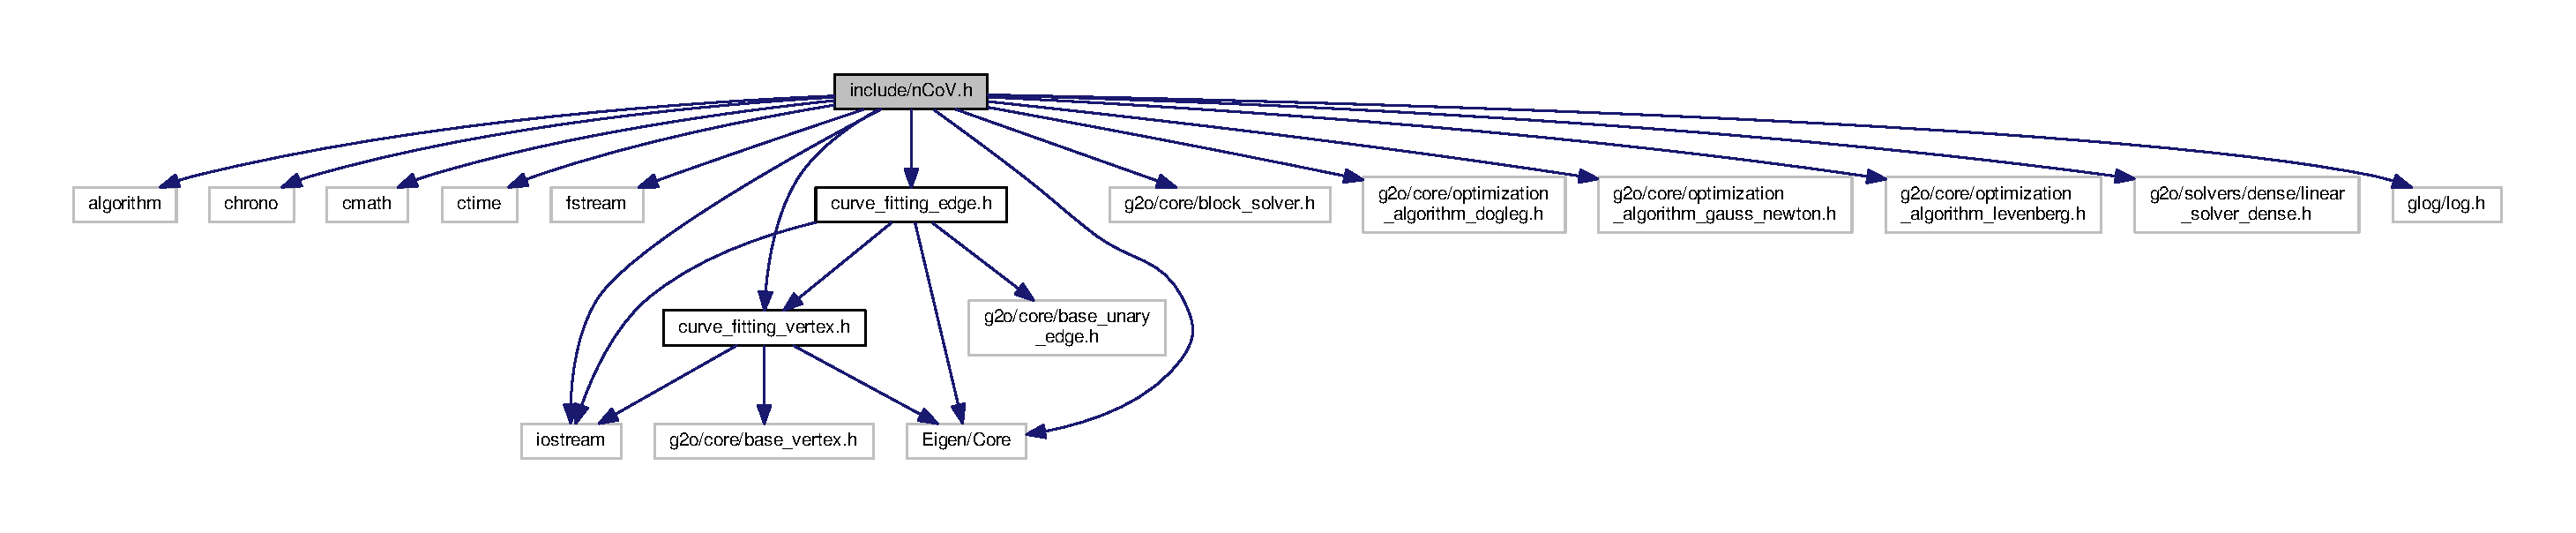
\includegraphics[width=350pt]{nCoV_8h__incl}
\end{center}
\end{figure}
This graph shows which files directly or indirectly include this file\+:\nopagebreak
\begin{figure}[H]
\begin{center}
\leavevmode
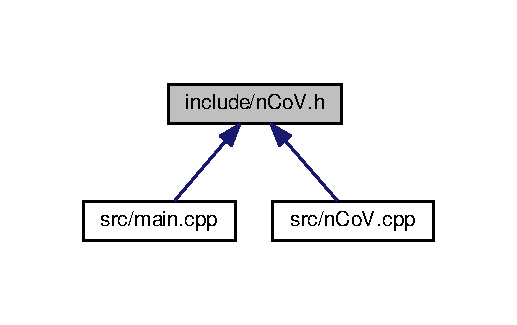
\includegraphics[width=248pt]{nCoV_8h__dep__incl}
\end{center}
\end{figure}
\subsection*{Classes}
\begin{DoxyCompactItemize}
\item 
class \hyperlink{classnCoV}{n\+CoV}
\end{DoxyCompactItemize}


\subsection{Detailed Description}
the \hyperlink{classnCoV}{n\+CoV} class declaration file 

\begin{DoxyAuthor}{Author}
Peripatetic\+Wind (\href{mailto:zhangzhihong@stu.xjtu.edu.cn}{\tt zhangzhihong@stu.\+xjtu.\+edu.\+cn}) 
\end{DoxyAuthor}
\begin{DoxyVersion}{Version}
1.\+0.\+0 
\end{DoxyVersion}
\begin{DoxyDate}{Date}
2020-\/02-\/10 22\+:43\+:22 
\end{DoxyDate}
\begin{DoxyParagraph}{Last\+Editor}
Peripatetic\+Wind 
\end{DoxyParagraph}
\begin{DoxyParagraph}{Last\+Edit\+Time}
2020-\/02-\/10 22\+:43\+:22 
\end{DoxyParagraph}
\begin{DoxyParagraph}{Email}
\href{mailto:zhangzhihong@stu.xjtu.edu.cn}{\tt zhangzhihong@stu.\+xjtu.\+edu.\+cn} 
\end{DoxyParagraph}
\begin{DoxyParagraph}{Company}
Xi\textquotesingle{}an Jiaotong University 
\end{DoxyParagraph}
\begin{DoxyCopyright}{Copyright}
Copyright (c) 2020 Peripatetic\+Wind. All rights reserved. 
\end{DoxyCopyright}
\begin{DoxyParagraph}{License}
Licensed under the M\+IT License. 
\end{DoxyParagraph}
\begin{DoxyParagraph}{Changelog}

\tabulinesep=1mm
\begin{longtabu} spread 0pt [c]{*4{|X[-1]}|}
\caption{Change Log}\label{_}\\
\hline
\rowcolor{\tableheadbgcolor}{\bf Date }&{\bf Version }&{\bf Author }&{\bf Description }\\\cline{1-4}
\endfirsthead
\hline
\endfoot
\hline
\rowcolor{\tableheadbgcolor}{\bf Date }&{\bf Version }&{\bf Author }&{\bf Description }\\\cline{1-4}
\endhead
2020-\/02-\/10 22\+:43\+:22 &1.\+0.\+0 &Peripatetic\+Wind &change log \\\cline{1-4}
\end{longtabu}

\end{DoxyParagraph}

\hypertarget{main_8cpp}{}\section{src/main.cpp File Reference}
\label{main_8cpp}\index{src/main.\+cpp@{src/main.\+cpp}}
{\ttfamily \#include $<$gflags/gflags.\+h$>$}\\*
{\ttfamily \#include \char`\"{}n\+Co\+V.\+h\char`\"{}}\\*
Include dependency graph for main.\+cpp\+:\nopagebreak
\begin{figure}[H]
\begin{center}
\leavevmode
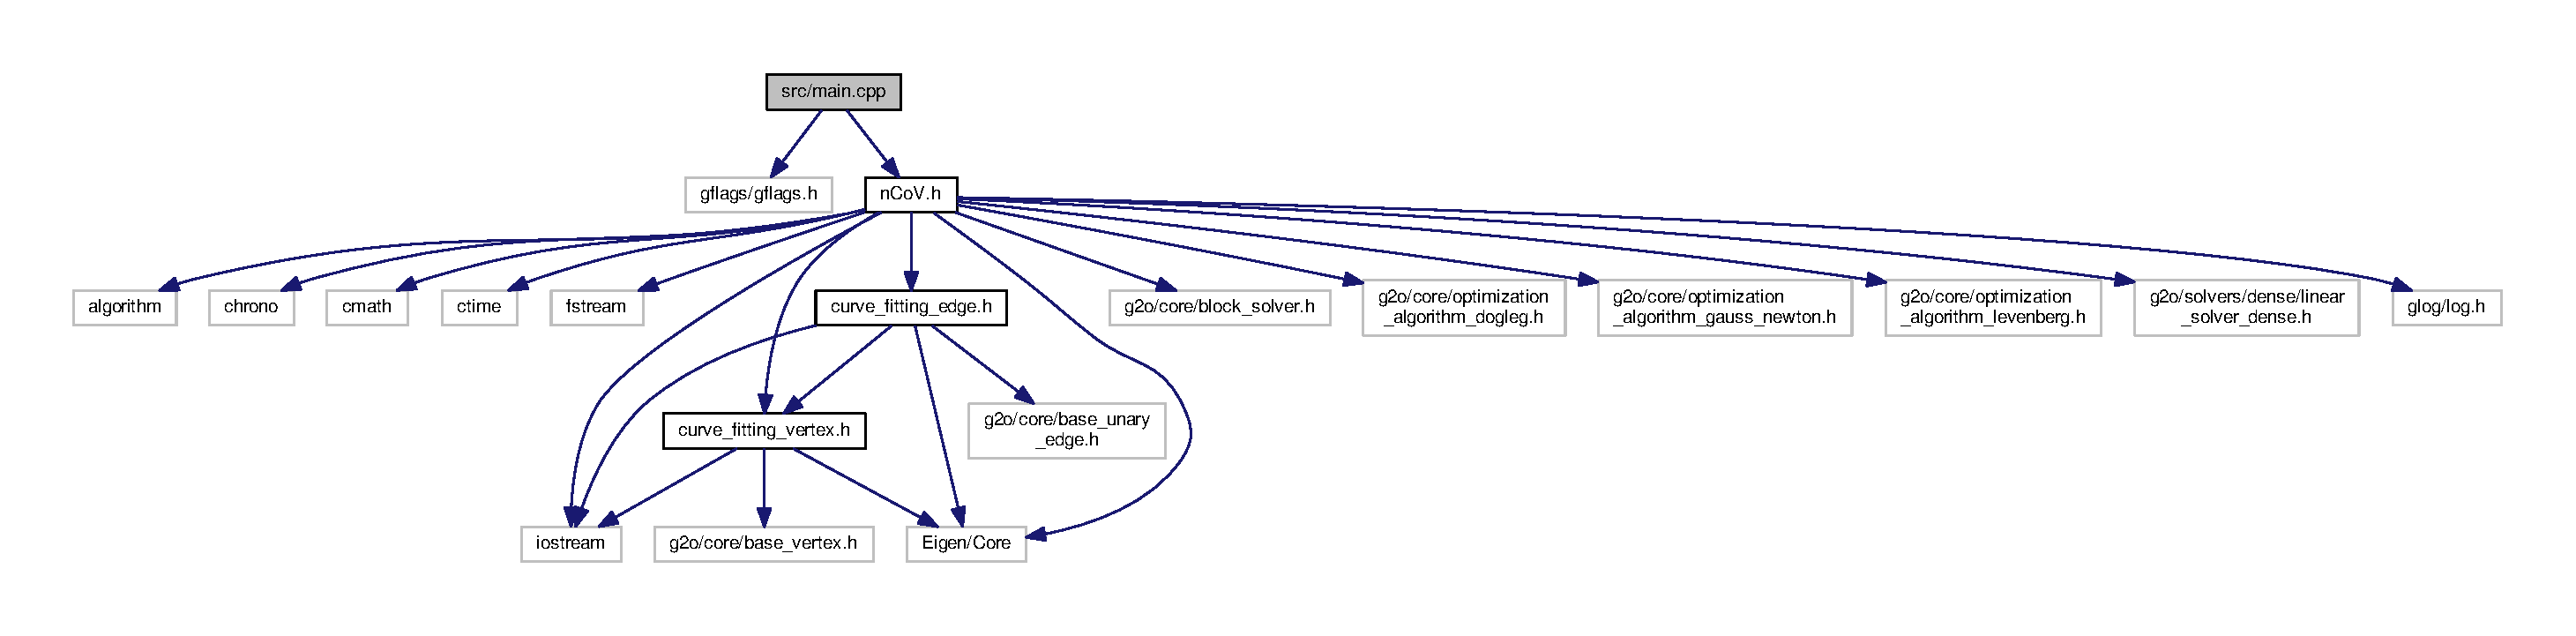
\includegraphics[width=350pt]{main_8cpp__incl}
\end{center}
\end{figure}
\subsection*{Functions}
\begin{DoxyCompactItemize}
\item 
\hyperlink{main_8cpp_ac61515ae4926c5ffeb447645eee3ac56}{D\+E\+F\+I\+N\+E\+\_\+int32} (d, 5,\char`\"{}the days to predict\char`\"{})
\begin{DoxyCompactList}\small\item\em 本程序用来预测每日感染人数 数据来源:http\+://m.medsci.\+cn/wh.asp \end{DoxyCompactList}\item 
int \hyperlink{main_8cpp_a3c04138a5bfe5d72780bb7e82a18e627}{main} (int argc, char $\ast$$\ast$argv)
\end{DoxyCompactItemize}


\subsection{Function Documentation}
\index{main.\+cpp@{main.\+cpp}!D\+E\+F\+I\+N\+E\+\_\+int32@{D\+E\+F\+I\+N\+E\+\_\+int32}}
\index{D\+E\+F\+I\+N\+E\+\_\+int32@{D\+E\+F\+I\+N\+E\+\_\+int32}!main.\+cpp@{main.\+cpp}}
\subsubsection[{\texorpdfstring{D\+E\+F\+I\+N\+E\+\_\+int32(d, 5,""the days to predict"")}{DEFINE_int32(d, 5,"the days to predict")}}]{\setlength{\rightskip}{0pt plus 5cm}D\+E\+F\+I\+N\+E\+\_\+int32 (
\begin{DoxyParamCaption}
\item[{d}]{, }
\item[{5}]{, }
\item[{\char`\"{}the days to predict\char`\"{}}]{}
\end{DoxyParamCaption}
)}\hypertarget{main_8cpp_ac61515ae4926c5ffeb447645eee3ac56}{}\label{main_8cpp_ac61515ae4926c5ffeb447645eee3ac56}


本程序用来预测每日感染人数 数据来源:http\+://m.medsci.\+cn/wh.asp 

\index{main.\+cpp@{main.\+cpp}!main@{main}}
\index{main@{main}!main.\+cpp@{main.\+cpp}}
\subsubsection[{\texorpdfstring{main(int argc, char $\ast$$\ast$argv)}{main(int argc, char **argv)}}]{\setlength{\rightskip}{0pt plus 5cm}int main (
\begin{DoxyParamCaption}
\item[{int}]{argc, }
\item[{char $\ast$$\ast$}]{argv}
\end{DoxyParamCaption}
)}\hypertarget{main_8cpp_a3c04138a5bfe5d72780bb7e82a18e627}{}\label{main_8cpp_a3c04138a5bfe5d72780bb7e82a18e627}

\hypertarget{nCoV_8cpp}{}\section{src/n\+CoV.cpp File Reference}
\label{nCoV_8cpp}\index{src/n\+Co\+V.\+cpp@{src/n\+Co\+V.\+cpp}}


the \hyperlink{classnCoV}{n\+CoV} class implementation file  


{\ttfamily \#include \char`\"{}n\+Co\+V.\+h\char`\"{}}\\*
Include dependency graph for n\+Co\+V.\+cpp\+:\nopagebreak
\begin{figure}[H]
\begin{center}
\leavevmode
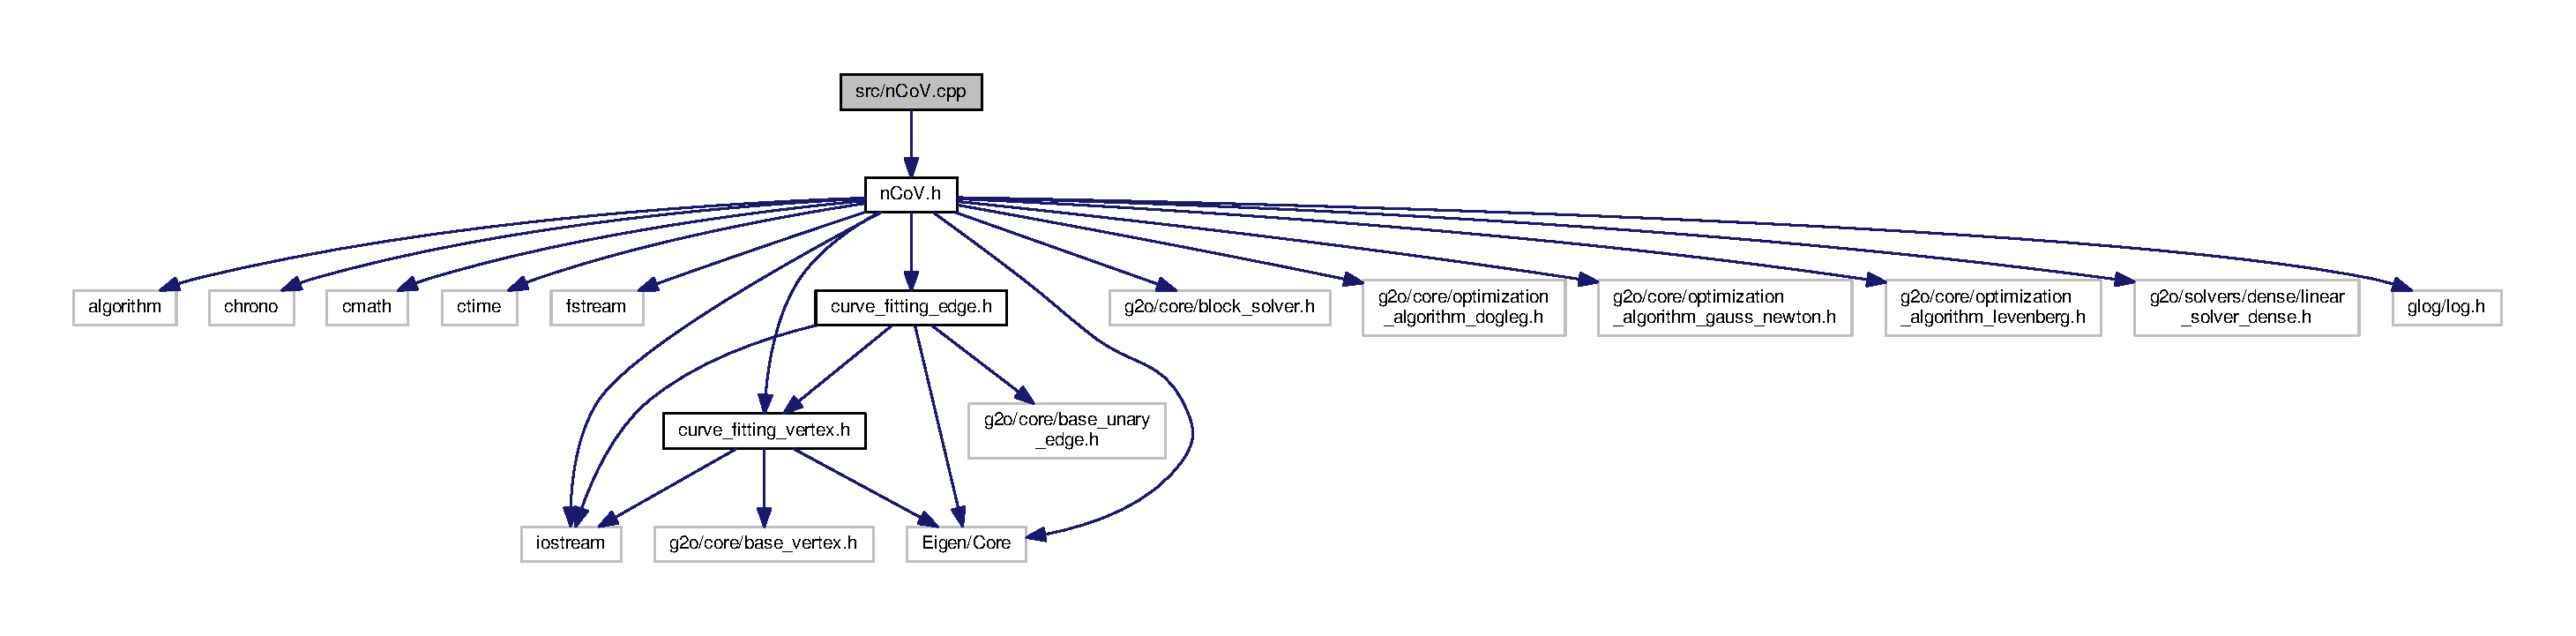
\includegraphics[width=350pt]{nCoV_8cpp__incl}
\end{center}
\end{figure}


\subsection{Detailed Description}
the \hyperlink{classnCoV}{n\+CoV} class implementation file 

\begin{DoxyAuthor}{Author}
Peripatetic\+Wind (\href{mailto:zhangzhihong@stu.xjtu.edu.cn}{\tt zhangzhihong@stu.\+xjtu.\+edu.\+cn}) 
\end{DoxyAuthor}
\begin{DoxyVersion}{Version}
1.\+0.\+0 
\end{DoxyVersion}
\begin{DoxyDate}{Date}
2020-\/02-\/10 22\+:43\+:01 
\end{DoxyDate}
\begin{DoxyParagraph}{Last\+Editor}
Peripatetic\+Wind 
\end{DoxyParagraph}
\begin{DoxyParagraph}{Last\+Edit\+Time}
2020-\/02-\/10 22\+:43\+:01 
\end{DoxyParagraph}
\begin{DoxyParagraph}{Email}
\href{mailto:zhangzhihong@stu.xjtu.edu.cn}{\tt zhangzhihong@stu.\+xjtu.\+edu.\+cn} 
\end{DoxyParagraph}
\begin{DoxyParagraph}{Company}
Xi\textquotesingle{}an Jiaotong University 
\end{DoxyParagraph}
\begin{DoxyCopyright}{Copyright}
Copyright (c) 2020 Peripatetic\+Wind. All rights reserved. 
\end{DoxyCopyright}
\begin{DoxyParagraph}{License}
Licensed under the M\+IT License. 
\end{DoxyParagraph}
\begin{DoxyParagraph}{Changelog}

\tabulinesep=1mm
\begin{longtabu} spread 0pt [c]{*4{|X[-1]}|}
\caption{Change Log}\label{_}\\
\hline
\rowcolor{\tableheadbgcolor}{\bf Date }&{\bf Version }&{\bf Author }&{\bf Description }\\\cline{1-4}
\endfirsthead
\hline
\endfoot
\hline
\rowcolor{\tableheadbgcolor}{\bf Date }&{\bf Version }&{\bf Author }&{\bf Description }\\\cline{1-4}
\endhead
2020-\/02-\/10 22\+:43\+:01 &1.\+0.\+0 &Peripatetic\+Wind &change log \\\cline{1-4}
\end{longtabu}

\end{DoxyParagraph}

%--- End generated contents ---

% Index
\backmatter
\newpage
\phantomsection
\clearemptydoublepage
\addcontentsline{toc}{chapter}{Index}
\printindex

\end{document}
